% Define document class
\documentclass[twocolumn]{aastex631}

% Filler text
\usepackage{blindtext}

% Begin!
\begin{document}

% Title
\title{\showyourwork: a workflow for open source scientific articles}

% Author list
\author[0000-0002-0296-3826]{Rodrigo Luger}

% Abstract with filler text
\begin{abstract}
    \blindtext
\end{abstract}

% Main body with filler text
\section{Introduction}
\Blindtext[4]


\begin{figure}[ht!]
    \begin{centering}
        \includegraphics[width=0.75\linewidth]{figures/HD118203_transit.pdf}
        \includegraphics[width=0.75\linewidth]{figures/HD118203_corner.pdf}
        \caption{
            Automatically-generated figures showing the transit of HD 118203b in \emph{TESS} (\emph{top}) and the joint posterior distributions over its period, radius, and impact parameter (\emph{bottom}). Both figures were generated from the same \texttt{Python} script in the \texttt{src/figures} directory (linked to in the \texttt{GitHub} icon in the margin). The other margin icon indicates that these figures depend on a dataset (a \texttt{.npz} file containing the posterior samples), 
            which is automatically generated by \showyourwork and uploaded to Zenodo. Users wishing to reproduce the results in this paper can choose whether to re-generate this dataset or download a static version from Zenodo (linked to in the margin).
        }
        \label{fig:HD118203}
    \end{centering}
\end{figure}

\begin{figure}[ht!]
    \begin{centering}
        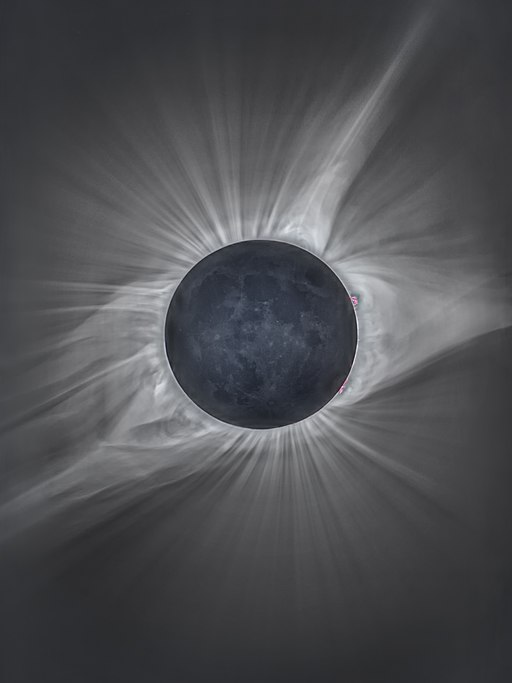
\includegraphics[width=0.75\linewidth]{static/eclipse.jpeg}
        \caption{
            A static figure committed to the repository showing a total solar eclipse. 
            Since this figure is in the \texttt{src/static} directory, \showyourwork knows not to attempt to generate it. 
            By default, margin icons are not added to static figures.
            Here we manually add icons linking to the original photograph on Wikimedia Commons and its license using the \texttt{\textbackslash marginicon} command.
        }
        \marginicon{%
            \stackon[3pt]{%
                \href{https://commons.wikimedia.org/wiki/File:Total\_Solar\_Eclipse\_8-21-17.jpg}{\color{sywBlue}\faWikipediaW}%
            }{%
                \href{https://commons.wikimedia.org/wiki/File:Total\_Solar\_Eclipse\_8-21-17.jpg\#Licensing}{\color{sywBlue}\faCreativeCommons}%
            }%
        }
        \label{fig:eclipse}
    \end{centering}
\end{figure}



\end{document}
